\section{Evolutionärer Algorithmus}\label{sec:evol-alg}
Für den Algorithmus wird angenommen,
dass die eine Liste der möglichen Spendetermine wie folgt eingegeben wird:
\begin{table}[ht]
    \begin{center}
        \begin{tabular}{l|c|c|c|c}
            PLZ     & Ort               &  Straße               & Datum     & Distanz   \\
            \hline
            12345   & Musterstadt       & Hauptstraße 42        & 5.3.2019  & 6.31      \\
            04711   & Beispieldorf      & Spenderstraße. 13     & 894.2019  & 20.42     \\
        \end{tabular}
    \end{center}
    \caption{Beispieldaten}
\end{table}


Der Algorithmus selbst benötigt hierbei lediglich das Datum und die Distanz.
Die anderen Merkmale dienen der finalen Darstellung für den Anwender.

Das Problem ähnelt stark dem bekannten \emph{Knappsackproblem}.
Dort wird versucht den Gesamtwert der mitgenommenen Gegenstände zu maximieren
und dabei die vorgegebenen Gewichtsgrenzen einzuhalten.

Entsprechend soll in dem hier beschriebenen Fall die Anzahl der besuchten Spendetermine unter
Einhaltung bestimmter Regeln maximiert werden.
Ergänzt wird dieses Problem durch die Minimierung der zurückgelegten Strecke.

\subsection{Genstring}
Wie auch bei einem Knappsackproblem üblich wird der Genstring als Bitstring modelliert.
Somit gilt:

\begin{equation}
    \label{eqn:genstring}
    \begin{split}
        x_i &\in \{ 0,1 \} \\
        x_i &= 1 \Rightarrow \text{Termin $i$ wird wahrgenommen} \\
        x   &= b_1b_2...b_n \in \{0,1\}^n\text{ mit $n = $ Anzahl der eingegebenen Termine}
    \end{split}
\end{equation}

\newpage
\subsection{Bewertungsfunktion}
Die Bewertungsfunktion hat das Ziel die Anzahl der besuchten Termine zu maximieren und die Gesamtstrecke zu minimieren.
Dies soll unter Beachtung der bereits vorgestellten Bedingungen geschehen.

Im Vergleich zu einer Produktionsplanung gibt es bei den Bedingungen keinen Spielraum.
In einer Produktionsplanung ist es möglicherweise gestattet die maximale Anzahl der Stunden zu überschreiten.
Dies wird in der Fitness entsprechend bestraft. Aber sollte das beste Ergebnis Überstunden enthalten ist es dennoch ein gültiges Ergebnis.

Die Bedingungen für das Blutspenden sind jedoch \enquote{harte} Bedingungen.
Das heißt, dass beispielsweise keine Spende möglich ist, wenn die letzte Spende erst 55 Tage her ist und nicht die geforderten 56.
Um solche Ergebnisse zu verhindern wird die Fitness für diese Gene auf $0$ gesetzt und nicht durch eine Bestrafung verringert.
Im weiteren Verlauf werden diese Gene aus der Population entfernt und können sich nicht reproduzieren.

Da die Anzahl der Spenden innerhalb von 12 Monaten geschlechterspezifisch ist,
fließt diese Zahl als Konstante $c$ in die Berechnung mit ein.

Die Anzahl der besuchten Termine und eine minimale Strecke sind zwei sich entgegenstehende Ziele.
Würde keiner Termine wahrgenommen werden, wäre die Gesamtstrecke $0$ und somit optimal.

Daher wird eine Gewichtung der beiden Merkmale durchgeführt.\linebreak
$w~\in~[0,1]$ steht hierbei für die Gewichtung der Anzahl besuchter Termine.
Entsprechend ist $(1-w)$ die Gewichtung der Strecke.
Um sicherzustellen, dass das Gewicht für beide Merkmale den gleichen Einfluss besitzt,
werden die jeweiligen Bewertungen auf den Bereich $[0,1]$ normiert.
Für die Anzahl geschieht dies durch eine Division mit $c$.

Das Normieren der Strecke ist hierbei komplexer.
Deren Bewertung wird mit $(1 - \frac{\sum x_i * d_i}{max(d)t* \sum x_i})$ berechnet.
Durch den Bruch wird der durchschnittliche Abstand zur maximal möglichen Strecke ($max(d)$) berechnet.
Am anschaulichsten erklärt sich diese Formel durch Betrachtung der Grenzfälle in \autoref{tab:grenzfaelle}
\begin{table}[ht]% Try here, and then top
    \begin{center}
        \begin{tabular}{l|c|c}
            Fall                            & $\cfrac{\sum x_i * d_i}{max(d) * \sum x_i}$  &  Bewertung \\
            \hline
            $\forall x_i = 1: d_i = max(d)$ & $1$                                           & $0$       \\
            $\forall x_i = 1: d_i = 0$      & $0$                                           & $1$       \\
        \end{tabular}
    \end{center}
    \caption{Grenzfälle Bewertung der Strecke}
    \label{tab:grenzfaelle}
  \end{table}

Insgesamt lässt sich die Fitness eines Gens nach Formel \ref{eqn:fitness} berechnen.
Die Funktion $B(x)$ bestimmt hierbei, ob die Nebenbedingungen erfüllt sind.

\begin{equation}
    \label{eqn:fitness}
    f(x)=
    \begin{cases}
        0,              & \text{wenn } B(x) = 0 \\
        w * \cfrac{\sum x_i}{c} + (1 - w) * \left(1 - \cfrac{\sum x_i * d_i}{max(d) * \sum x_i}\right) & \text{sonst}
    \end{cases}
\end{equation}

\ref{eqn:bedingung} stellt die Bedingungen dar.
$t_i$ steht hierbei für das Datum eines Spendetermins.
$t_j - t_i <= 1y$ ist wahr, wenn der Abstand zwischen den beiden Terminen höchstens ein Jahr ist.
$t_j - t_i < 56d$ ist wahr, wenn der Abstand kleiner als 56 Tage ist.
Ist das Ergebnis $1$ so gelten die Bedingungen als erfüllt.



\begin{multline}
    \label{eqn:bedingung}
    B(x)=
    \begin{cases}
        0, & \text{wenn } \exists x_i \in x : x_i = 1  \wedge \\
           & \hspace{10ex} \lvert \{ x_j\in x \mid x_j = 1 \wedge i < j \wedge t_j - t_i <= 1y  \} \rvert > c   \\
        0, & \text{wenn } \exists x_i, x_j \in x : \left( (x_i = x_j = 1) \wedge (i < j) \wedge (t_j - t_i < 56d) \right)    \\
        1  & \text{sonst}
    \end{cases}
\end{multline}

Durch die verhältnismäßig strengen Bedingungen ist mit einer hohen Anzahl an ungültigen Genen zu rechnen.
Kompensiert wird dies durch eine große Population um ausreichend \enquote{gesunde} Gene zur späteren Evolution zu erhalten.




\subsection{Kombination}\label{sec:evol-alg-kombi}
Zwei Gene werden durch einen sogenannten \emph{1-Point Crossover} \cite{AJ2015} kombiniert.
Hierzu werden die Bitstrings der Eltern an einer zufälligen Stelle getrennt und die Teilstrings untereinander getauscht.
Folgende Tabelle zeigt beispielhaft den Crossover an Position 4 von zwei Bitstrings der Länge 9:

\begin{table}[ht]
    \begin{center}
        \begin{tabular}{l c}
            Elternteil 1 & \colorbox{lime!30}{$1010$~}$\mid$\colorbox{lime!30}{ $10010$} \\
            Elternteil 2 & \colorbox{cyan!30}{$1011$~}$\mid$\colorbox{cyan!30}{ $10110$} \\
            \hline
            Kind 1       & \colorbox{lime!30}{$1010$~}$\mid$\colorbox{cyan!30}{ $10110$} \\
            Kind 2       & \colorbox{cyan!30}{$1011$~}$\mid$\colorbox{lime!30}{ $10010$} \\
        \end{tabular}
    \end{center}
    \caption{1-Point Crossover (nach \cite{AJ2015})}
\end{table}

Die Auswahl der zu kombinierenden Eltern geschieht durch eine \emph{Tournament Selection} mit vier Teilnehmern.
Wie in \autoref{fig:tournament} dargestellt werden erst jeweils zwei der vier Teilnehmer miteinander verglichen.
Jeweils die besten beiden werden anschließend nochmal miteinander verglichen um den Sieger zu ermittelt.

\begin{figure}[h]
    \centering
    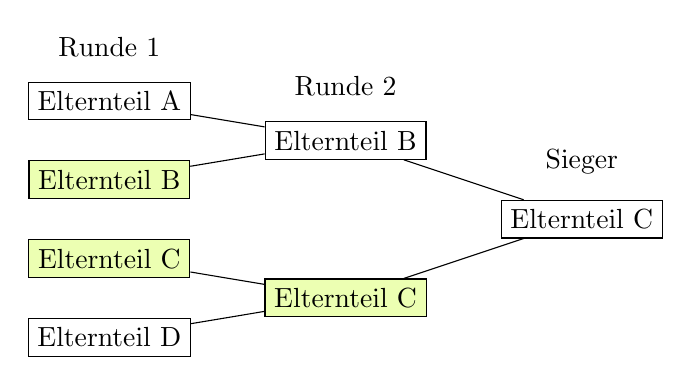
\begin{tikzpicture}
        [
           every node/.style={rectangle,draw},
           level distance=3cm
        ]
        \tikzstyle{level 1}=[sibling distance=20mm]
        \tikzstyle{level 2}=[sibling distance=10mm]
        \node[label={[label distance=0.2cm]90:Sieger}] {Elternteil C} [grow'=left]
        child {node[fill=lime!30]{Elternteil C}
            child {node{Elternteil D}}
            child {node[fill=lime!30]{Elternteil C}}
        }
        child {node[label={[label distance=0.2cm]90:Runde 2}]{Elternteil B}
            child {node[fill=lime!30]{Elternteil B}}
            child {node[label={[label distance=0.2cm]90:Runde 1}]{Elternteil A}}
        };
    \end{tikzpicture}
    \caption{Beispiel eines Tournament}
    \label{fig:tournament}
\end{figure}

\subsection{Mutationen}
In einem Knappsackproblem ist eine zufällige Bitinversion eine übliche Mutation.
Für das Blutspende-Problem bringt dies mit sehr hoher Wahrscheinlichkeit
eine Reduktion der Fitness mit sich.

Wird ein aktives Bit deaktiviert, so sinkt damit die Anzahl der wahrgenommenen Termine und damit die Fitness.
Wird ein inaktives Bit aktiviert, so ist die Wahrscheinlichkeit hoch, dass eine der Bedingungen verletzt wird.

Daher wird zur Mutation kein Bit invertiert, sondern zufällig ein aktives Bit in seiner unmittelbaren Nachbarschaft verschoben.
Die Weite und Richtung der Verschiebung werden zufällig ermittelt. Als maximal mögliche Verschiebung wird die Schrittweite angenommen.
Diese wird initial gesetzt und mittels der $\frac{1}{5}$-Regel iterativ angepasst.

Die Regel besagt, dass die Schrittweite erhöht wird, falls mehr als $\frac{1}{5}$ der Mutationen besser sind als ihre Ursprungs-Gene
und verringert wird, falls weniger als $\frac{1}{5}$ erfolgreich sind.
Um sicherzustellen, dass jederzeit eine Mutation möglich ist, wird die Schrittweite nach unten auf $1$ beschränkt.

Da positive Bits nur verschoben und keine negativen Bits aktiviert werden,
erhöht sich die Anzahl der besuchten Termine nicht durch die Mutation.
Dies ist jedoch mit der vorherigen Rekombination zweier Gene möglich.

\subsection{Initiale Population}
Initial wird die Population erzeugt,
indem für jedes Gen drei zufällige Bits gesetzt werden.
Um die Wahrscheinlichkeit zu reduzieren, dass diese Bits zu Nah zueinander sind,
wird der Genstring in 3 gleich große Bereiche aufgeteilt.
Aus jedem dieser Bereiche wird anschließend ein Bit zufällig gewählt.

Zum Vergleich wurden 100-mal jeweils Populationen von 1000 Genen mit beiden Verfahren erzeugt.
Der Versuch zeigt, dass ohne diese Beschränkung lediglich etwa 35\% der Gene die Bedingungen erfüllen.
Die Beschränkung hebt den Anteil der gültigen Gene auf etwa 80\%.

Die dennoch hohe Anzahl an ungültigen Genen hat den Nachteil,
dass anfangs nur wenige \enquote{nützliche} Gene zur Verfügung stehen.
Dies wird durch eine hohe Populationszahl kompensiert.
Ein prototypisches Programm, welches in \autoref{sec:prototyp} vorgestellt wird,
zeigt, dass eine Population von 500 hierfür ausreicht.

\subsection{Evolution}
Die Evolution geschieht unter folgenden Regeln.
Die entsprechenden Parameter können im Programm angegeben werden.
\begin{itemize}
    \item Eine \emph{Elite} der fittesten Gene \enquote{überlebt} eine Generation
    \item Die restlichen Gene der nächsten Generation werden durch Kombination erzeugt.
    \begin{itemize}
        \item Hierfür kommen nach dem in \autoref{sec:evol-alg-kombi} vorgestellten Verfahren alle Gene der aktuellen Generation in Frage.
        \item Zusätzlich wird ein neu erzeugtes Gen mit einer gewissen Wahrscheinlichkeit mutiert.
    \end{itemize}
    \item Nach Kombination und Mutation werden alle Gene, welche nicht die Bedingungen erfüllen aus der Population entfernt.
    \item Der gesamte Algorithmus endet, wenn die durchschnittliche und die beste Fitness mit gegebener Präzision identisch sind oder spätestens nach einer maximalen Anzahl von Durchläufen.
\end{itemize}

\noindent
In \autoref{sec:prototyp} - \autoref{tab:parameter} sind die praktisch genutzten Parameter aufgeführt.

\subsection{Pareto-Front}
Eine maximale Anzahl von Terminen und eine minimale Gesamtstrecke sind zwei entgegengesetzte Ziele.

Bezüglich der Strecke wäre es am optimalsten keinen Termin wahrzunehmen,
da so die Gesamtstrecke mit $0$ minimal ist.
Ebenso muss eine Strecke in Kauf genommen werden,
wenn die maximal mögliche Anzahl von Terminen besucht werden soll.

Hat man die maximale Anzahl von Terminen mit einer -- unter diesen Bedingungen -- minimalen Gesamtstrecke erreicht,
so lässt sich die Strecke nur noch verringern, indem die Anzahl der Termine verringert wird.

Wenn die Fitness eines Aspekts nur noch verbessert werden kann,
wenn sich im Gegenzug die Fitness eines anderen Aspekts verschlechtert,
wird dies \emph{Pareto-Front} genannt.

\begin{figure}[h]
    \centering
    \includegraphics[width=0.65\textwidth]{pareto.png}
    \caption{Beispiel einer Pareto-Front \cite{Paretofr62:online}}
    \label{fig:pareto}
\end{figure}

Eine mögliche Darstellung der Pareto-Front zeigt \autoref{fig:pareto}.
Zum Beispiel ist $f1$ die Fitness der Anzahl und $f2$ die Fitness der Strecke.
In diesem Programmentwurf lässt sich mittels der Gewichtung steuern,
in welchem Bereich der Pareto-Front eine Lösung gesucht wird.
Je stärker die Anzahl gewichtet wird, desto weiter Links befindet sich die Lösung in diesem Schaubild.
